%%%%%%%%%%%%%%%%%%%%%%%%%%% asme2ej.tex %%%%%%%%%%%%%%%%%%%%%%%%%%%%%%%
% Template for producing ASME-format journal articles using LaTeX    %
% Written by   Harry H. Cheng, Professor and Director                %
%              Integration Engineering Laboratory                    %
%              Department of Mechanical and Aeronautical Engineering %
%              University of California                              %
%              Davis, CA 95616                                       %
%              Tel: (530) 752-5020 (office)                          %
%                   (530) 752-1028 (lab)                             %
%              Fax: (530) 752-4158                                   %
%              Email: hhcheng@ucdavis.edu                            %
%              WWW:   http://iel.ucdavis.edu/people/cheng.html       %
%              May 7, 1994                                           %
% Modified: February 16, 2001 by Harry H. Cheng                      %
% Modified: January  01, 2003 by Geoffrey R. Shiflett                %
% Butchered: October 15, 2014 by John Karasinski                %
% Use at your own risk, send complaints to /dev/null                 %
%%%%%%%%%%%%%%%%%%%%%%%%%%%%%%%%%%%%%%%%%%%%%%%%%%%%%%%%%%%%%%%%%%%%%%

%%% use twocolumn and 10pt options with the asme2ej format
\documentclass[twocolumn,10pt]{asme2ej}

\usepackage{epsfig} %% for loading postscript figures
\usepackage{listings}
\usepackage{amsmath}
\usepackage{graphicx}
\usepackage{grffile}
\usepackage{pdfpages}

%% The class has several options
%  onecolumn/twocolumn - format for one or two columns per page
%  10pt/11pt/12pt - use 10, 11, or 12 point font
%  oneside/twoside - format for oneside/twosided printing
%  final/draft - format for final/draft copy
%  cleanfoot - take out copyright info in footer leave page number
%  cleanhead - take out the conference banner on the title page
%  titlepage/notitlepage - put in titlepage or leave out titlepage
%  
%% The default is oneside, onecolumn, 10pt, final

\title{Case Study \# 1: 1D Transient Heat Diffusion}

%%% first author
\author{John Karasinski
    \affiliation{
	Graduate Student Researcher\\
	Center for Human/Robotics/Vehicle Integration and Performance\\
	Department of Mechanical Engineering\\
	University of California\\
	Davis, California 95616\\
    Email: karasinski@ucdavis.edu
    }	
}

\begin{document}
\maketitle    

%%%%%%%%%%%%%%%%%%%%%%%%%%%%%%%%%%%%%%%%%%%%%%%%%%%%%%%%%%%%%%%%%%%%%%
\section{Problem Description}

The problem of 1D unsteady heat diffusion in a slab of unit length with a zero initial temperature and both ends maintained at a unit temperature can be described by:
\begin{equation}
\frac{\partial T}{\partial t} = \frac{\partial^2T}{\partial x^2} \mbox{ subject to } \left\{ \begin{array}{lll}
        \mbox{$T(x, 0^-)= 0 $} & \mbox{for } &0 \leq x \leq 1 \\
        \mbox{$T(0, t) = T(1, t) = 1$} & \mbox{for } &t > 0 \end{array} \right.
\label{eq_DEF}
\end{equation}
\noindent and has the well known analytical solution:
\begin{equation}
\begin{split}
T^*(x,t) = 1 - \sum\limits_{k=1}^\infty \frac{4}{(2k-1)\pi} & \sin[(2k-1)\pi x] \star \\
		    &  \exp[-(2k-1)^2\pi^2t].
\end{split}
\end{equation}

%%%%%%%%%%%%%%%%%%%%%%%%%%%%%%%%%%%%%%%%%%%%%%%%%%%%%%%%%%%%%%%%%%%%%%
\section{Solution Algorithms}

The Taylor-series (TS) method can be used on this equation to derive a finite difference approximation to the PDE. Applying the definition of the derivative, 
\begin{equation}
f'(x) \approx \frac{f(x + \epsilon) - f(x)}{\epsilon}
\end{equation}

\noindent to Eqn.~(\ref{eq_DEF}) yields:
\begin{equation}
\begin{split}
\frac{\partial T}{\partial t} = & \frac{T(x, t + \Delta t) - T(x,t)}{\Delta t} \\
				      = & \frac{T_{i}^{k+1} - T_{i}^{k}}{\Delta t}
\end{split}
\end{equation}

From the definition of the Taylor series,
\begin{equation}
f(x+\epsilon) = f(x) + \epsilon f'(x) + \frac{\epsilon^2}{2} f''(x) + ...
\end{equation}
\noindent which, when applied to $T_{i}^{k+1}$  and $T_{i}^{k}$ gives:
\begin{equation}
T_{i+1} = T_i + \Delta x \frac{\partial T_i}{\partial x} + \frac{\Delta x^2}{2} \frac{\partial^2 T_i}{\partial x^2} + \mathcal{O}(\Delta x^3)
\label{eq_ADD1}
\end{equation}
\noindent and
\begin{equation}
T_{i-1} = T_i - \Delta x \frac{\partial T_i}{\partial x} + \frac{\Delta x^2}{2} \frac{\partial^2 T_i}{\partial x^2} - \mathcal{O}(\Delta x^3)
\label{eq_ADD2}
\end{equation}

Adding Eqn.~(\ref{eq_ADD1}) and Eqn.~(\ref{eq_ADD2}) yields:
\begin{equation}
T_{i+1} + T_{i-1} = 2T_i + \Delta x^2 \frac{\partial^2 T_i}{\partial x^2} + \mathcal{O}(\Delta x^4)
\end{equation}
\noindent we can also combine the approximation for the second order term from Eqn.~(\ref{eq_DEF}) to find
\begin{equation}
\frac{\partial^2 T}{\partial x^2} = \frac{T_{i+1} + 2T_{i} + T_{i-1}}{\Delta x^2} + \mathcal{O}(\Delta x^4),
\end{equation}
\noindent which we can combine withe the above equations to form
\begin{equation}
\frac{T_i^{k+1}-T_i^k}{\Delta t} \approx \frac{T_{i+1}^k - 2T_i^k + T_{i-1}^k}{\Delta x^2}
\end{equation}

This result can be arranged to form both Forward-Time, Centered-Space (FTCS) explicit and implicit schemes. Rearranging, the explicit scheme is:
\begin{equation}
T_i^{k+1} = sT_{i+1}^k +(1- 2s)T_i^k + sT_{i}^k
\end{equation}
\noindent and the implicit scheme is
\begin{equation}
T_i^k = -sT_{i+1}^{k+1} +(1+2s)T_i^{k+1} - sT_{i-1}^k
\end{equation}
\noindent where
\begin{equation}
s = \frac{\alpha \Delta t}{\Delta x^2}
\end{equation}
\noindent and $\alpha$ is the thermal diffusivity of the material.

%%%%%%%%%%%%%%%%%%%%%%%%%%%%%%%%%%%%%%%%%%%%%%%%%%%%%%%%%%%%%%%%%%%%%%
\section{Results}

A Python script was used to obtain results for a 21 point mesh (N=21), and the Root Mean Square error,
\begin{equation}
\mbox{RMS} = \frac{1}{N}\sqrt{\sum\limits_{i=1}^N[T_i^n - T^*(x_i, t_n)]^2}
\end{equation}
was obtained for $s(=\Delta t/ \Delta x^2)$ = 1/6, 0.25, 0.5, and 0.75, at $t$ = 0.03, 0.06, and 0.09.

%%%%%%%%%%%%%%%%%%%%%%%%%%%%%%%%%%%%%%%%%%%%%%%%%%%%%%%%%%%%%%%%%%%%%%
%%%%%%%%%%%%%%% begin table   %%%%%%%%%%%%%%%%%%%%%%%%%%
\begin{table}[t]
%\caption{Figure and table captions do not end with a period}
\begin{center}
\label{table_ASME}
\begin{tabular}{|c c | c c|}
\hline
s & t & Implicit RMS & Explicit RMS \\
\hline
1/6 & 0.03 & 7.27E-4 & 9.25E-3\\
1/6 & 0.06 & 6.99E-5 & 1.19E-2\\
1/6 & 0.09 & 1.98E-4 & 1.31E-2\\
\hline
0.25 & 0.03 & 4.70E-4 & 1.38E-2\\
0.25 & 0.06 & 1.27E-4 & 1.90E-2\\
0.25 & 0.09 & 1.96E-4 & 2.02E-2\\
\hline
0.5 & 0.03 & 7.92E-4 & 3.66E-2\\
0.5 & 0.06 & 3.20E-4 & 4.71E-2\\
0.5 & 0.09 & 4.10E-4 & 4.63E-2\\
\hline
0.75 & 0.03 & 1.13E-3 & 8.13E-2 \\
0.75 & 0.06 & 5.17E-4 & 8.83E-2\\
0.75 & 0.09 & 6.22E-4 & 7.38E-2 \\
\hline
\end{tabular}
\caption{RMS results from the numerical simulations compared to the analytic solution}
\end{center}
\end{table}

%%%%%%%%%%%%%%%% end table %%%%%%%%%%%%%%%%%%% 
%%%%%%%%%%%%%%%%%%%%%%%%%%%%%%%%%%%%%%%%%%%%%%%%%%%%%%%%%%%%%%%%%%%%%%

The RMS between the implicit and analytic solutions and the explicit and analytic solutions are shown in Table~\ref{table_ASME}. The RMS tended to grow as a function of $s$, and shrink as a function of $t$. Additionally, the RMS for the explicit solution tended to be two orders of magnitude larger than the RMS for the implicit solution.

\begin{figure}[htb]
\begin{center}
\includegraphics[width=0.5\textwidth]{../figures/proj_1_s_0.166_t_0.03.pdf}
\includegraphics[width=0.5\textwidth]{../figures/proj_1_s_0.166_t_0.06.pdf}
\includegraphics[width=0.5\textwidth]{../figures/proj_1_s_0.166_t_0.09.pdf}
\caption{Results for $s = 1/6$}
\end{center}
\end{figure}

\begin{figure}[htb]
\begin{center}
\includegraphics[width=0.5\textwidth]{../figures/proj_1_s_0.25_t_0.03.pdf}
\includegraphics[width=0.5\textwidth]{../figures/proj_1_s_0.25_t_0.06.pdf}
\includegraphics[width=0.5\textwidth]{../figures/proj_1_s_0.25_t_0.09.pdf}
\caption{Results for $s = 0.25$}
\end{center}
\end{figure}

\begin{figure}[htb]
\begin{center}
\includegraphics[width=0.5\textwidth]{../figures/proj_1_s_0.5_t_0.03.pdf}
\includegraphics[width=0.5\textwidth]{../figures/proj_1_s_0.5_t_0.06.pdf}
\includegraphics[width=0.5\textwidth]{../figures/proj_1_s_0.5_t_0.09.pdf}
\caption{Results for $s = 0.5$}
\end{center}
\end{figure}

\begin{figure}[htb]
\begin{center}
\includegraphics[width=0.5\textwidth]{../figures/proj_1_s_0.75_t_0.03.pdf}
\includegraphics[width=0.5\textwidth]{../figures/proj_1_s_0.75_t_0.06.pdf}
\includegraphics[width=0.5\textwidth]{../figures/proj_1_s_0.75_t_0.09.pdf}
\caption{Results for $s = 0.75$}
\end{center}
\end{figure}
%%%%%%%%%%%%%%%%%%%%%%%%%%%%%%%%%%%%%%%%%%%%%%%%%%%%%%%%%%%%%%%%%%%%%%
\section{Discussions}
Shankle chicken tail, fatback short ribs meatball pancetta ball tip sirloin short loin. Pork tongue pork belly pork loin beef ribs. Shank turkey pork belly pork loin ham hock ball tip leberkas meatloaf chuck ground round filet mignon kielbasa sirloin turducken tri-tip. Pancetta brisket sirloin beef ribs spare ribs, swine bacon ham hock. Ham kielbasa corned beef turkey turducken. Kevin biltong pork, tenderloin chuck pig ball tip filet mignon.

%%%%%%%%%%%%%%%%%%%%%%%%%%%%%%%%%%%%%%%%%%%%%%%%%%%%%%%%%%%%%%%%%%%%%%
% The bibliography is stored in an external database file
% in the BibTeX format (file_name.bib).  The bibliography is
% created by the following command and it will appear in this
% position in the document. You may, of course, create your
% own bibliography by using thebibliography environment as in
%
% \begin{thebibliography}{12}
% ...
% \bibitem{itemreference} D. E. Knudsen.
% {\em 1966 World Bnus Almanac.}
% {Permafrost Press, Novosibirsk.}
% ...
% \end{thebibliography}

% Here's where you specify the bibliography style file.
% The full file name for the bibliography style file 
% used for an ASME paper is asmems4.bst.
%\bibliographystyle{asmems4}

% Here's where you specify the bibliography database file.
% The full file name of the bibliography database for this
% article is asme2e.bib. The name for your database is up
% to you.
%\bibliography{asme2e}

%%%%%%%%%%%%%%%%%%%%%%%%%%%%%%%%%%%%%%%%%%%%%%%%%%%%%%%%%%%%%%%%%%%%%%
\clearpage
\onecolumn
\appendix       %%% starting appendix
\section*{Appendix A: Python Code}

\begin{figure}[b]
\begin{center}
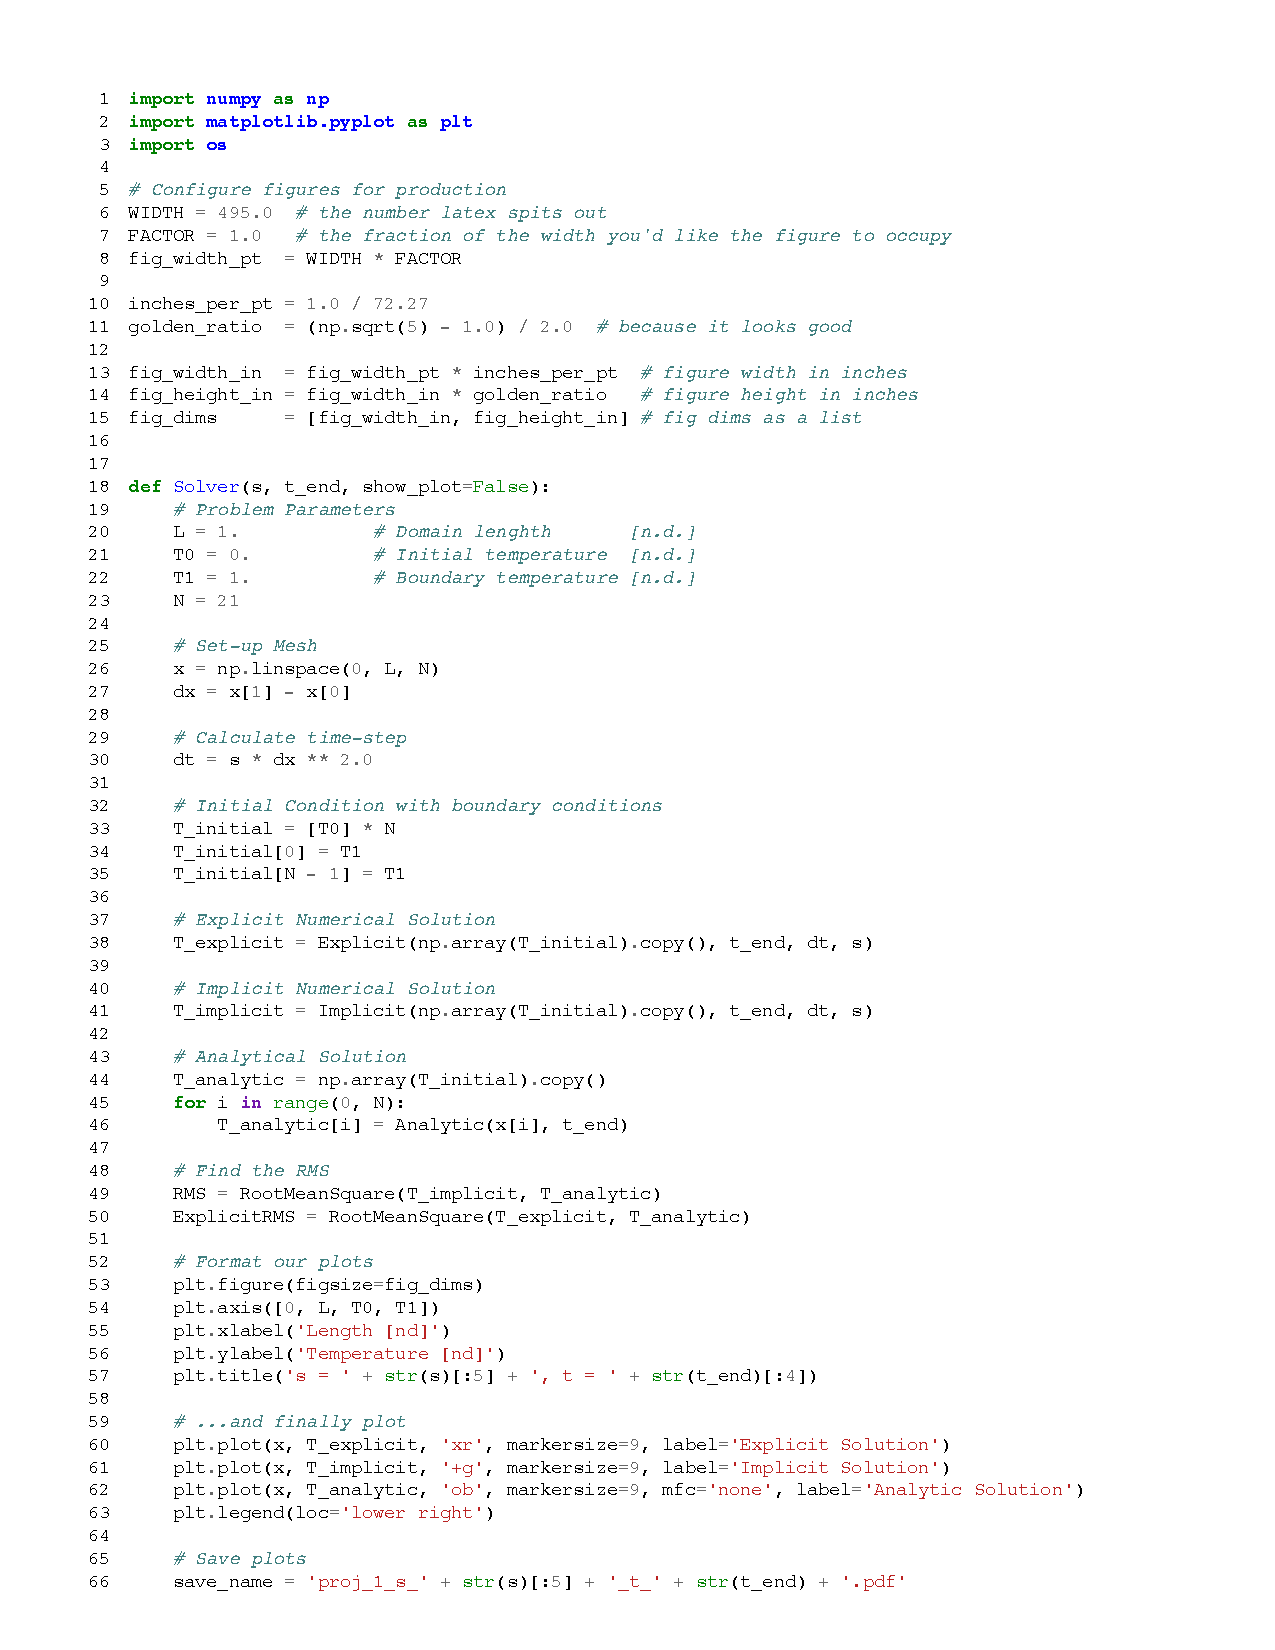
\includegraphics[page=1,width=0.93\textwidth]{../Karasinski - Case Study 1.pdf}
\end{center}
\end{figure}

\begin{figure}[htb]
\begin{center}
\includegraphics[page=2,width=0.93\textwidth]{../Karasinski - Case Study 1.pdf}
\end{center}
\end{figure}

\begin{figure}[htb]
\begin{center}
\includegraphics[page=3,width=0.93\textwidth]{../Karasinski - Case Study 1.pdf}
\end{center}
\end{figure}

\begin{figure}[htb]
\begin{center}
\includegraphics[page=4,width=0.93\textwidth]{../Karasinski - Case Study 1.pdf}
\end{center}
\end{figure}
%%%%%%%%%%%%%%%%%%%%%%%%%%%%%%%%%%%%%%%%%%%%%%%%%%%%%%%%%%%%%%%%%%%%%%
%\section*{Appendix B: Head of Second Appendix}
%\subsection*{Subsection head in appendix}
%The equation counter is not reset in an appendix and the numbers will
%follow one continual sequence from the beginning of the article to the very end as shown in the following example.
%\begin{equation}
%a = b + c.
%\end{equation}

\end{document}
